\documentclass[12pt,a4paper]{article}

\PassOptionsToPackage{
  backend=biber,
  style=numeric, % eller authoryear
  sorting=nyt,
  giveninits=true,
  maxbibnames=99,
  doi=false,isbn=false,url=true,
  dashed=false
}{biblatex}


\usepackage{preamble}
\usepackage{xcolor}


\addbibresource{./referanser.bib}

% ------ Metadata ------
\newcommand{\institution}{FHS/Cyberingeniørskolen}
\newcommand{\laboratory}{Matematiske Metoder 2}
\newcommand{\coursecode}{ING2501}
\newcommand{\assignmenttype}{PROSJEKTRAPPORT 1}
\newcommand{\assignmenttitle}{Telegrafligningen}
\newcommand{\studentnameA}{Abay, Yonatan Monken}
\newcommand{\studentnameB}{Aleksandersen, Tor Johan Drange}
\newcommand{\studentnameC}{Bertilsson, Agnes Liv}
\newcommand{\studentnameD}{Bjørdal, Olav Schei}
\newcommand{\studentnameE}{Vesteng, Karen}
\newcommand{\partnername}{Ola Nordmann}
\newcommand{\class}{VING 78}
\newcommand{\submissiondate}{\today}

\begin{document}

% frontpage.tex
\thispagestyle{empty}
\begin{minipage}{0.15\textwidth}
    
\includegraphics[height=3cm]{Media/cisk.png}
\end{minipage}%
\begin{minipage}{0.4\textwidth}
    \vspace{10ex}
    \raggedright
    {\bfseries\itshape\institution}\\
    {\bfseries\itshape\laboratory}
\end{minipage}%
\begin{minipage}{0.4\textwidth}
    \vspace{13ex}
    \raggedleft
    {\today}
\end{minipage}
\vspace{1ex}

{\noindent\rule{\textwidth}{2pt}} \\ \vspace{3ex}
\begin{center}
    {\fontsize{32}{36}\selectfont \bfseries \assignmenttype}\\[6ex]
    {\fontsize{22}{26}\selectfont \bfseries \assignmenttitle}\\[10ex]
    {\fontsize{16}{20}\selectfont \bfseries {\coursecode}}\\[3ex]

    {\noindent\rule{\textwidth}{2pt}} \\\vspace{5ex}

    {\fontsize{20}{24}\selectfont \bfseries AV}\\[3ex]
    {\fontsize{20}{24}\selectfont \bfseries \studentnameA}\\ [2ex]
    {\fontsize{20}{24}\selectfont \bfseries \studentnameB}\\ [2ex]
    {\fontsize{20}{24}\selectfont \bfseries \studentnameC}\\ [2ex]
    {\fontsize{20}{24}\selectfont \bfseries \studentnameD}\\ [2ex]
    {\fontsize{20}{24}\selectfont \bfseries \studentnameE}\\ [2ex]
\end{center}

{\noindent\rule{\textwidth}{2pt}} \\\vspace{5ex}

\begin{flushleft}
    \begin{tabular}{@{}ll}
    {\fontsize{14}{18}\selectfont \bfseries KLASSE:} & {\fontsize{14}{18}\selectfont \bfseries \class} \\
    \vspace{16ex} \\
    {\fontsize{14}{18}\selectfont \bfseries Rapport levert:} & {\fontsize{14}{18}\selectfont \bfseries \submissiondate} \\
    \end{tabular}
\end{flushleft}
\clearpage


\pagenumbering{Roman}
\setcounter{page}{1}

\section*{Sammendrag}
Denne rapporten undersøker hvordan telegrafligningen kan brukes til å modellere signalforplantning i elektriske transmisjonslinjer. I rapporten ble det lagt spesiell vekt på forplantningen i koaksialkabler. Formålet har vært å forstå hvordan demping og dispersjon påvirker signalets form og kvalitet, spesielt når signalene må bevege seg over en lengre distanse. Vi har sammenlignet teoretiske modeller med praktiske målinger for å underbygge konklusjonen. 
\\[1em]
Arbeidet består av en teoretisk del hvor telegrafligningen utledes fra Kirchhoffs lover, og hvor begrepene demping, faseforskyvning og dispersjon analyseres ved hjelp av Fourier-metoder. Deretter ble en rekke numeriske modeller utviklet i Python for å simulere signalforløp. Dette ble vist gjennom modeller av transmisjonslinjer som spenner fra ideelle, tapsfrie tilfeller til realistiske modeller med både demping og dispersjon. Resultatene fra simuleringene ble sammenlignet med laboratoriemålinger av firkantpulser sendt gjennom koaksialkabler med lengdene 5m og 30m. Forvrengningene i disse kablene ble sammenliknet med en koaksialkabel på 1m.
\\[1em]
Resultatene viser at signalet i korte kabler i hovedsak bevarer formen sin, mens lengre kabler gir tydeligere demping av høyfrekvente komponenter og økt pulsbredding. Den teoretiske modellen basert på telegrafligningen beskriver disse effektene godt, og forklarer hvorfor praktiske standarder som Ethernet setter en øvre grense på kabellengde.


\clearpage

\tableofcontents
\clearpage

\pagenumbering{arabic}
\setcounter{page}{1}

\section{Innledning}

Utviklingen av elektrisk kommunikasjon på 1800-tallet skapte et behov for å forstå hvordan 
signaler forplantet seg i lange ledningsnettverk. Telegrafen, som var den første teknologien 
for rask kommunikasjon over store avstander, ble raskt bygget ut både i Europa og USA. Etter hvert 
som ledningsnettene ble lengre, oppsto praktiske problemer: signalene ble svakere, de ble 
forsinket, og de kunne endre form. For å løse disse utfordringene måtte man utvikle en matematisk 
modell som tok hensyn til de fysiske egenskapene til en elektrisk ledning.
\\[1em]
Oliver Heaviside, en britisk fysiker og ingeniør, brukte Maxwells ligninger som utgangspunkt og 
formulerte på slutten av 1800-tallet det som i dag kalles \textit{telegrafligningen}. Den beskriver 
hvordan spenning og strøm endrer seg i tid og rom langs en elektrisk linje, idét 
resistans, induktans, kapasitans og konduktans inkluderes i modellen. Telegrafligningen ble et viktig teoretisk verktøy 
for å forstå og forbedre kvaliteten på telegraf- og telefonlinjer, og den la grunnlaget for hele 
transmisjonslinjeteorien som fortsatt brukes i moderne elektronikk og telekommunikasjon \cite{geeksforgeeks_telegrapher}.
\\[1em]
I dag er de samme prinsippene fortsatt aktuelle. Ethernetkabler, coaxialkabler og telefonlinjer kan modelleres 
som transmisjonslinjer, der signalet påvirkes av tap og dispersjon. Ethernet-standarden setter en 
maksimal kabellengde på 100 meter for å sikre at signalet kan overføres uten for store tap og 
forvrengninger. Coaxialkablers maksimale lengde uten stort tap av signalkvalitet vil også variere basert på frekvensene som brukes. På samme måte mister lange telefonkabler kvalitet, spesielt når de brukes til høyere 
frekvenser som i bredbånd (DSL). Begge disse fenomenene kan forklares gjennom telegrafligningen.
\\[1em]
I denne rapporten tar vi derfor utgangspunkt i telegrafligningen som matematisk modell og gjennom numerisk
modellering og simulering, og laboratorietester undersøker vi hvordan signaler oppfører seg i korte og 
lange ledningsnettverk ved forskjellige frekvenser. Vi vil også se på hvordan ulike parametere påvirker 
signalets kvalitet, med demping, faseendring og forvrengning som sentrale temaer. Dette gir oss en bedre forståelse av
hvordan elektriske signaler oppfører seg i praksis. 
\clearpage




\section{Teori}

    \textbf{Motivasjon og sammenheng:} For å forstå hvorfor det er en grense på 100 meter for Ethernet-kabler, og hvordan signaler dempes og forvrenges i slike kabler, bruker vi telegrafligningen. Denne beskriver hvordan elektriske signaler forplanter seg i transmisjonslinjer, og gir oss verktøyene til å analysere tap, dispersjon.

\subsection{Kirchhoffs lover}

Grunnlaget for telegrafligningen ligger i Kirchhoffs lover, som beskriver hvordan spenning og strøm 
fordeler seg i elektriske kretser. Disse lovene er direkte basert på fysikkens bevaringsprinsipper 
for energi og ladning, og de brukes til å beskrive forholdet mellom elektriske størrelser i ethvert 
kretsnettverk.

\textbf{Kirchhoffs spenningslov (KVL)} sier at summen av alle spenningsendringer rundt en lukket 
sløyfe er lik null. Dette uttrykker energibevaring: den elektriske energien som brukes opp i motstander 
og spoler, må være lik den energien som tilføres av spenningskilder. I telegrafligningen brukes KVL 
til å uttrykke hvordan spenningen endrer seg langs et lite element av ledningen. Spenningsfallet 
langs et element avhenger av den ohmske motstanden og induktansen, og beskrives matematisk som
\begin{equation}
\frac{\partial u}{\partial x} = -R i - L \frac{\partial i}{\partial t}.
\end{equation}

\textbf{Kirchhoffs strømlov (KCL)} sier at summen av alle strømmene som går inn i et knutepunkt, 
er lik summen av de som går ut. Dette er et uttrykk for ladningsbevaring. I telegrafligningen brukes 
KCL til å beskrive hvordan strømmen endrer seg langs ledningen, når en del av strømmen lekker til jord 
gjennom konduktans og kapasitans. Dette gir
\begin{equation}
\frac{\partial i}{\partial x} = -G u - C \frac{\partial u}{\partial t}.
\end{equation}

Ved å kombinere Kirchhoffs lover kan man beskrive hvordan både spenning og strøm endrer seg 
langs ledningen over tid. Dette er utgangspunktet for telegrafligningen, som gir 
en fullstendig matematisk modell for hvordan signaler forplanter seg, dempes og forvrenges når de beveger 
seg gjennom en elektrisk leder.

\subsection{Fourierrekker}

Mange signaler kan brytes ned i sine frekvenskomponenter ved hjelp av Fourier-analyse. Dette er spesielt nyttig i signalbehandling og for å forstå hvordan ulike frekvenser påvirkes av transmisjonslinjen. Ethernet-signaler kan sees på som en sekvens av pulser (bitstrøm), som i praksis kan betraktes som et periodisk pulstog. Dette gjør at Fourierrekker er et naturlig verktøy for å analysere slike signaler i frekvensdomenet, siden pulstoget kan uttrykkes som en sum av sinus- og cosinuskomponenter.\\[1em]
En periodisk funksjon $f(t)$ med periode $T$ kan uttrykkes som en Fourier-rekke:
\begin{equation}
f(t) = a_0 + \sum_{n=1}^{\infty} \left( a_n \cos\left(\frac{2\pi n t}{T}\right) + b_n \sin\left(\frac{2\pi n t}{T}\right) \right)
\end{equation}
med koeffisienter gitt ved:
\begin{align*}
a_0 &= \frac{1}{T} \int_{0}^{T} f(t) \, dt \\
a_n &= \frac{2}{T} \int_{0}^{T} f(t) \cos\left(\frac{2\pi n t}{T}\right) dt \\
b_n &= \frac{2}{T} \int_{0}^{T} f(t) \sin\left(\frac{2\pi n t}{T}\right) dt
\end{align*}
I Kompleks form:
\begin{equation}
f(t) = \sum_{n=-\infty}^{\infty} c_n e^{j \frac{2\pi n t}{T}}, \quad \text{der} \quad c_n = \frac{1}{T} \int_{-T/2}^{T/2} f(t) e^{-j \frac{2\pi n t}{T}} dt, \quad c_0 = \frac{1}{T} \int_{-T/2}^{T/2} f(t) dt
\end{equation}
I dette prosjektet vil vi bruke Fourier-analyse for å dekomponere Ethernet-signaler i sine frekvenskomponenter, slik at vi kan studere hvordan hver komponent påvirkes av transmisjonslinjens egenskaper.
Ved å gjennomføre målinger for forskjellige kabellengder, kan vi sammenligne de målte dataene med de teoretiske prediksjonene basert på Fourier-analyse og telegraflikningen.
Vi får da overføringsfunksjonen for kabelen.
\begin{equation}
    H(f) = \frac{V_{out}(f)}{V_{in}(f)}
\end{equation}
Som beskriver hvordan signalet endres i frekvensdomenet når det passerer gjennom kabelen.
Denne analysen hjelper oss å forstå hvordan ulike frekvenskomponenter dempes og forvrenges, noe som er avgjørende for å forklare begrensningen på kabelens lengde.
Setter vi inn overførsingsfunksjonen i komplekse Fourier-rekken, kan vi modellere hvordan hele signalet endres når det går gjennom kabelen.
\begin{equation}
    f_{out}(t) = \sum_{n=-\infty}^{\infty} H\left(\frac{n}{T}\right) c_n e^{j \frac{2\pi n t}{T}}
\end{equation}
\subsection{Telegraflikningen og transmisjonslinjer}
En transmisjonslinje kan beskrives ved fire per-enhet-lengde parametre:
\begin{itemize}
    \item $R$ \, [$\Omega$/m] \,-- motstand (ledertap),
    \item $L$ \, [H/m] \,-- induktans (magnetisk lagring),
    \item $C$ \, [F/m] \,-- kapasitans (elektrisk lagring),
    \item $G$ \, [S/m] \,-- ledningsevne (lekkasjetap).
\end{itemize}
Ved å kombinere Kirchhoffs lover med disse parameterne utledes telegrafligningen, som beskriver spenning og strøm som funksjon av både posisjon og tid langs kabelen. For spenningen $u(x,t)$ kan den skrives på formen:
\begin{equation}
    u_{tt} + \left(\frac{R}{L} + \frac{G}{C}\right)u_t + \left(\frac{RG}{LC}\right)\,u = \left(\frac{1}{LC}\right) u_{xx}
\end{equation}
\[
    u_{tt} + \left(\alpha + \beta\right)u_t + \alpha\beta\,u = c^2 u_{xx}, \qquad \alpha=\frac{R}{L}, \qquad \beta=\frac{G}{C}, \qquad c = \frac{1}{\sqrt{LC}} ,
\]
der $u(x,t)$ er spenningen langs kabelen og $c$ er utbredelseshastigheten i kabelen.  
Denne ligningen viser at et signal ikke bare forplanter seg med en hastighet bestemt av $L$ og $C$, men også blir dempet og forvrengt på grunn av $R$ og $G$. Resultatet er at høyfrekvente komponenter i signalet svekkes og spres mer enn lave frekvenser, noe som over tid fører til \emph{demping og dispersjon}.  
Ethernet-signaler består ikke av rene sinusbølger, men av pulser med et bredt spekter av frekvenser. Mens Fourier-analyse kan hjelpe oss  å uttrykke signalet som en sum av ulike frekvenskomponenter, gir telegrafligningen oss verktøy til å studere hvordan hver enkelt komponent påvirkes. Dermed kan vi forklare hvorfor en grense på omtrent 100 meter er praktisk: etter denne lengden er tapet og forvrengningen så store at signalet ikke lenger kan tolkes pålitelig av mottakeren.


\subsubsection{R - Resistans}
Resistans per lengde $[\Omega/\mathrm{m}]$ er den ohmske motstanden i lederen. Den skyldes av materialets resistivitet og ledertverrsnitt, og øker med temperatur. Motstanden øker dempingen og reduserer rekkevidden til signalet. I telegrafligningen bidrar R direkte til tidsdemping av både strøm og spenning.

\subsubsection{L - Induktans}
Induktansen per lengde $[\mathrm{H}/\mathrm{m}]$ er magnetisk lagring av energi rundt lederen når strømmen endres, per meter kabel. Sammen med kapasitans vil denne bestemme farten på signalet i kabelen. I linjemodellen står induktansen i serie.

\subsubsection{C - Kapasitans}
Kapasitans per lengde $[\mathrm{F}/\mathrm{m}]$ er elektrisk lagring av energi i feltet mellom leder og referanse, per meter. Sammen med induktans har kapasitans påvirkning på fart. I linjemodellen er dette en gren til jord, den trekker ladning når spenningen endres.

\subsubsection{G - Shunt-ledningsevne (lekkasje)}
$G$ $[\mathrm{S}/\mathrm{m}]$ er shunt-ledningsevnen til jord per lengdeenhet. Den modellerer dielektrisk lekkasje gjennom isolasjonen og står parallelt med kapasitansen $C$ i linjemodellen. Større $G$ gir større demping fordi mer energi tappes i dielektrikumet. Høy fuktighet, aldring eller skadet/dårlig isolasjon øker $G$ (ideell isolasjon gir $G \approx 0$).

\clearpage
\subsubsection{Utledning av telegraflikningen}
Telegraflikningen kan utledes ved å analysere en liten del av transmisjonslinjen, som vist i figuren nedenfor. Vi betrakter et segment av linjen med lengde $\Delta x$, og bruker Kirchhoffs spennings- og strømlov for å sette opp differensialligninger for spenning og strøm.
\begin{figure}[h]
    \centering
    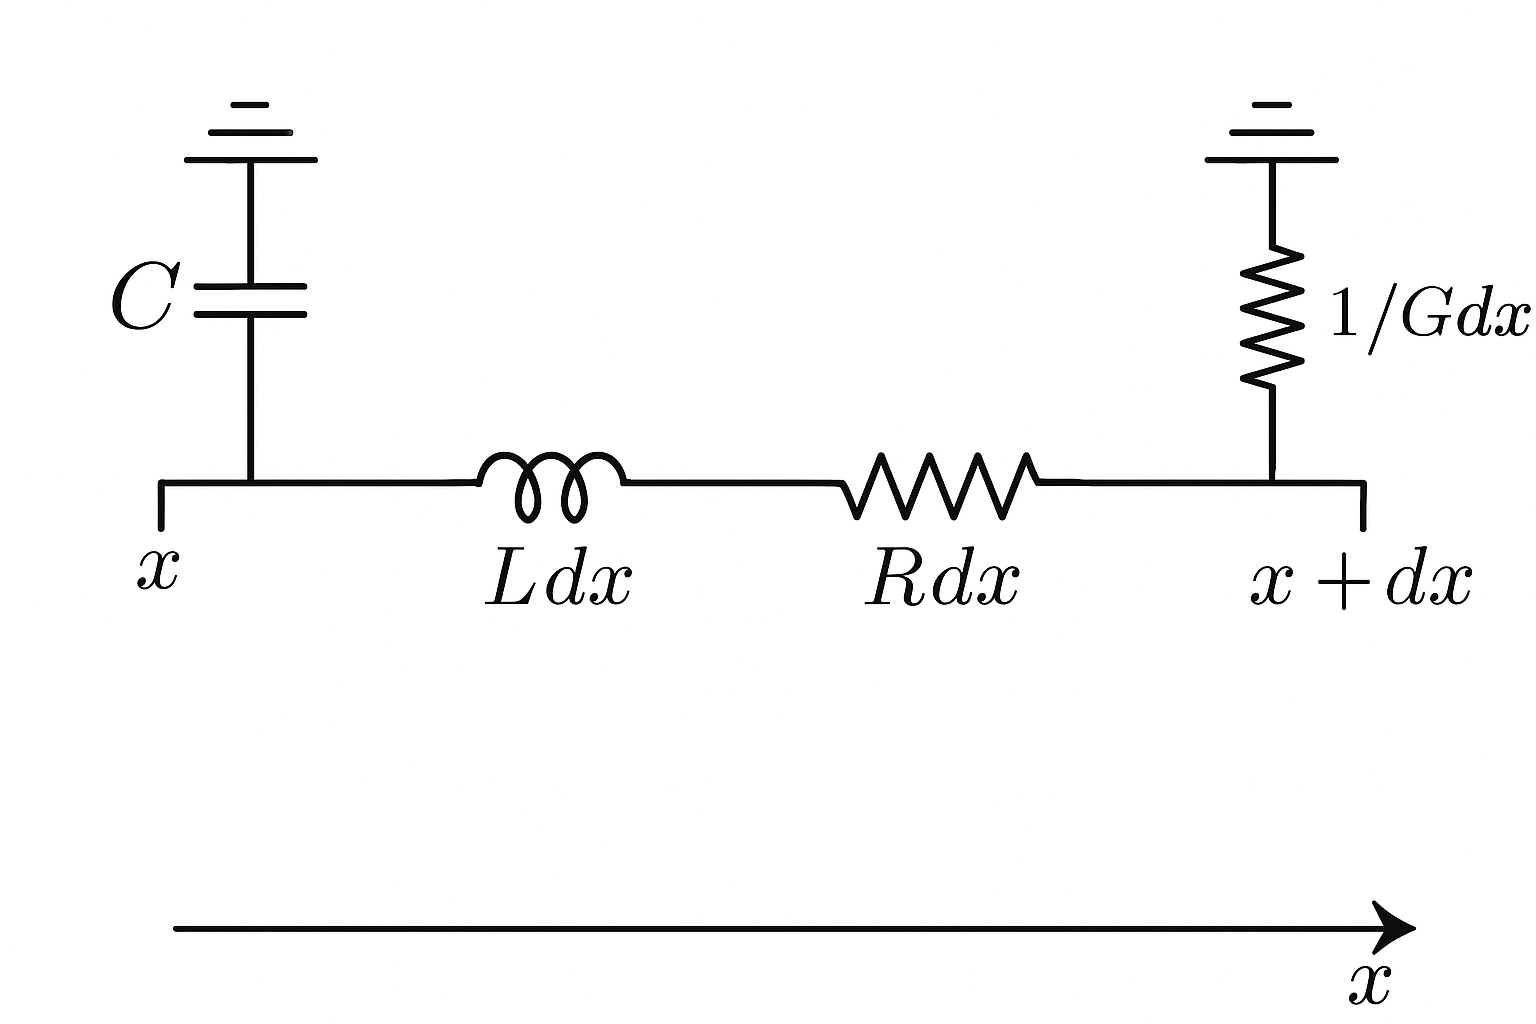
\includegraphics[width=0.6\textwidth]{Media/telegraflinje.png}
    \caption{Elementært segment av en transmisjonslinje med per-enhet-lengde parametere.}
    \label{fig:transmission_line_segment}   
\end{figure}\\
Ved å anvende Kirchhoffs spenningslov på segmentet får vi:
\[
    u(x,t) - u(x+\Delta x,t) = R \Delta x \cdot i(x,t) + L \Delta x \cdot \frac{\partial i(x,t)}{\partial t} .
\]
Ved å dele begge sider av ligningen med $\Delta x$ og lar $\Delta x \to 0$ får vi den første differensialligningen:
\begin{equation}
    \frac{\partial u(x,t)}{\partial x} = -R i(x,t) - L \frac{\partial i(x,t)}{\partial t} . 
\end{equation}
Tilsvarende, ved å bruke Kirchhoffs strømlov, får vi:
\[
    i(x,t) - i(x+\Delta x,t) = -G \Delta x \cdot u(x,t) - C \Delta x \cdot \frac{\partial u(x,t)}{\partial t} .
\]
Igjen, ved å dele begge sider av ligningen med $\Delta x$ og lar $\Delta x \to 0$ får vi den andre differensialligningen:
\[
    \frac{\partial i(x,t)}{\partial x} = -G u(x,t) - C \frac{\partial u(x,t)}{\partial t} .
\]
Ved å derivere den første ligningen med hensyn på $x$ og den andre med hensyn på $t$, og deretter eliminere $i(x,t)$, får vi telegraflikningen for spenningen:
\[
    u_{tt} + \left(\frac{R}{L} + \frac{G}{C}\right)u_t + \left(\frac{RG}{LC}\right)\,u = \left(\frac{1}{LC}\right) u_{xx}
\]
\clearpage
\noindent Dette kan vi skrive som:
\begin{equation}
    u_{tt} + (\alpha + \beta)u_t + \alpha \beta u = c^2 u_{xx}, \qquad c = \frac{1}{\sqrt{LC}} ,
    \label{eq:telegraflikningen}
\end{equation}
der vi har definert:
\[
    \alpha = \frac{R}{L}, \qquad \beta = \frac{G}{C} .
\]
Dette er en dampet bølgeligning som beskriver hvordan spenningen forplanter seg langs transmisjonslinjen, med demping og forvrengning bestemt av parametrene $R$, $L$, $C$, og $G$.



\subsubsection{Propagerende løsning og overføringsfunksjon}

I forrige del utledet vi telegraflikningen for spenning langs en kabel uttrykt ved de per-lengde-parametrene $R, L, G, C$ som beskriver hvordan spenningen varierer både i tid og rom \eqref{eq:telegraflikningen}. Denne likningen er en såkalt bølgelikning med demping. Vi forventer derfor at løsningene skal ha bølgekarakter som oscillerer i tid og samtidig forplanter seg langs kabelen. For å fange dette opp antar vi en løsning på formen
\begin{equation}
V(x,t) = \Re\!\left\{ U e^{j\omega t - \gamma(\omega)x} \right\}.
\label{eq:harm-ansatz}
\end{equation}
Her har vi valgt tre elementer:
\begin{itemize}
    \item \textbf{Tidsdelen $e^{j\omega t}$:} beskriver en harmonisk oscillasjon i tid. At vi bruker den 
    komplekse eksponentialen i stedet for $\cos(\omega t)$ eller $\sin(\omega t)$ skyldes at dette 
    gjør beregningene enklere. Til slutt tar vi realdelen for å hente ut det fysiske signalet.
    \item \textbf{Romdelen $e^{-\gamma x}$:} beskriver hvordan signalet utvikler seg langs kabelens lengde. 
    Hvis $\gamma$ er reell, betyr dette ren demping. Hvis $\gamma$ er imaginær, betyr det ren faseforskyvning. 
    I praksis er $\gamma$ kompleks, slik at vi får begge deler.
    \item \textbf{Kompleks amplitude $U$:} setter størrelsen og fasen på bølgen.\\
\end{itemize}
Dette kalles en \emph{harmonisk ansats}. Den er valgt fordi vi vet fra Fourier-teori at alle signaler 
kan bygges opp som en sum av slike harmoniske komponenter. Når vi kjenner kabelens respons på en frekvens, 
kan vi utvide til vilkårlige signaler. Setter vi \eqref{eq:harm-ansatz} inn i telegraflikningen \eqref{eq:telegraflikningen}:
\[    
    V_{tt} + (\alpha + \beta)V_{t} + \alpha \beta V = c^2 V_{xx}.
\]
Ser vi at den tidslige avledningen bare gir faktorer av $j\omega$:
\[
    V_{t} = j\omega V, \quad V_{tt} = -\omega^2 V,
\]
og den romlige avledningen gir faktorer av $\gamma$:
\[
    V_{x} = -\gamma V, \quad V_{xx} = \gamma^2 V.
\]
Som gir oss:
\[    
-\omega^2 V + j\omega(\alpha+\beta)V + \alpha \beta V = c^2 \gamma^2 V.
\]
Vi kan forkorte med $V$ (som er forskjellig fra null) og får:
\[
c^2 \gamma^2(\omega) = \alpha \beta - \omega^2 + j\omega(\alpha+\beta).
\]
\clearpage
Dette er en såkalt \emph{dispersjonsrelasjon}, som forteller hvilke kombinasjoner av 
frekvens $\omega$ og bølgetall $\gamma$ som er mulige. Vi kan løse for $\gamma$ og får
\[
\gamma(\omega) = \frac{1}{c}\sqrt{\alpha\beta - \omega^2 + j\omega(\alpha+\beta)}.
\]
Setter vi inn definisjonene på $\alpha,\beta$ og $c$, kan dette skrives på den standardformen
som brukes i transmisjonslinjeteori:
\begin{equation}
\;\gamma(\omega) = \sqrt{(R+j\omega L)(G+j\omega C)}\;
\label{eq:prop-konstant}
\end{equation}
Dette uttrykket viser tydelig hvordan både ledertap ($R$) og dielektriske tap ($G$) bidrar 
til at signalet dempes, mens $L$ og $C$ bestemmer hastigheten til bølgen. Vi kan også uttrykke $\gamma$
i form av sin reelle og imaginære del:
\[
\gamma(\omega) = \alpha_p(\omega) + j\beta_p(\omega).
\]
Her har $\alpha_p(\omega)$ enheten Np/m (neper per meter) og forteller hvor raskt amplituden 
avtar med lengden, mens $\beta_p(\omega)$ har enheten rad/m og forteller hvor raskt fasen 
øker langs kabelen. Fra $\beta_p$ kan vi utlede bølgens fasehastighet:
\[v_p = \frac{\omega}{\beta_p}\]
og dermed hvor stor tidsforsinkelse signalet får etter en viss lengde.\\[1em]
Hvis vi nå ser på en kabel av lengde $l$, vil en harmonisk komponent ved frekvens $\omega$ 
endres med faktoren
\begin{equation}
H(\omega,l) = e^{-\gamma(\omega)l} = e^{-\alpha_p(\omega)l}\,e^{-j\beta_p(\omega)l}
\end{equation}
Dette er kabelens \emph{overføringsfunksjon}. 
Den kan forstås slik:
\begin{itemize}
    \item $e^{-\alpha_p l}$: amplituden reduseres eksponentielt med lengden, 
    \item $e^{-j\beta_p l}$: signalet forskyves i fase, tilsvarende en tidsforsinkelse.\\[1em]
\end{itemize}
Så langt har vi bare sett på en harmonisk bølge. Men i praksis er alle signaler satt sammen av mange slike bølger. 
Et vilkårlig innsignal kan skrives som en Fourier-rekke:
\[
f_{\text{in}}(t) = \sum_n c_n e^{j\omega_n t}.
\]
etter kabelen vil hver komponent være påvirket av $H(\omega_n,l)$, og vi får
\[
f_{\text{out}}(t) = \sum_n H(\omega_n,l)\,c_n e^{j\omega_n t}.
\]
Dermed virker kabelen som et frekvensavhengig filter: lave frekvenser slipper nesten uendret gjennom, 
mens høye frekvenser dempes kraftig. For firkantsignaler betyr dette at de skarpe kantene, 
som består av mange høye frekvenser, gradvis blir avrundet etter hvert som lengden øker. 
Det er nettopp dette vi kan observere i laboratoriet når vi sender firkantpulser gjennom en Ethernet-kabel.

\clearpage
\subsection{Demping (amplituderespons)}
Demping beskrives av realdelen av propagasjonskonstanten:
\[ 
  \alpha_p(\omega)=\Re\{\gamma(\omega)\}
\]
Den sier noe om hvor stor faktor hver frekvenskomponent dempes i amplitude. Denne faktoren er definert som størrelsen av overføringsfunksjonen:
\[
|H(\omega,l)|=e^{-\alpha_p(\omega)\,l}, \qquad |H(\omega,l)|_{\mathrm{dB}} = 20\log_{10}|H| = -8.686\,\alpha_p(\omega)\,l
\]
Når $c_n$ er Fourier-koeffisienten til n-te harmoniske komponent, er amplituden til denne komponenten etter kabelen gitt ved:
\[
|c_n^{out}| = |H(\omega_n,l)| \cdot |c _n| = e^{-\alpha_p(\omega_n) l} |c_n|
\]
Hvorfor signalet dempes kan forklares med to hovedmekanismer:\\
\begin{itemize}[leftmargin=2.8em,style=nextline]
  \item \textbf{Skinneffekt}: Når frekvensen øker, presses strømmen mot overflaten av lederen. Det effektive tverrsnittet blir mindre, og den elektriske motstanden per lengde øker. For runde ledere (og godt approksimert i praksis) gjelder:
  \[
  R(\omega)\ \propto\ \sqrt{\omega}
  \]
  Ut fra propagasjonskonstanten \eqref{eq:prop-konstant} følger at $\alpha_p(\omega)$ vokser omtrent som $\sqrt{\omega}$.\\
  \item \textbf{Dielektriske tap}: Et virkelig dielektrikum er ikke tapsfritt: polarisasjonen henger litt etter feltet (faseforsinkelse), noe som kan modelleres med \emph{loss tangent} \(\tan\delta\). For små tap får vi den nyttige tilnærmingen
  \[
  G(\omega)\ =\ \omega\,C\,\tan\delta \quad \Rightarrow \quad G(\omega)\ \propto\ \omega
  \]
  slik at tapet øker lineært med frekvens. Dette bidrar også til \(\alpha_p(\omega)\) og dermed til økende demping med \(\omega\).\\
\end{itemize}
\clearpage

Dette gir da direkte utslag i overføringsfunksjonen. Siden både \(R(\omega)\) og \(G(\omega)\) øker med frekvens, dempes høyfrekvente komponenter mest.
I tid betyr det sløvere kanter og “droop” på platået (vertikal lukking i øyediagram) siden høye frekvenser som trengs for å gjenskape skarpe kanter, er mest dempet.
\begin{figure}[h]
    \centering
    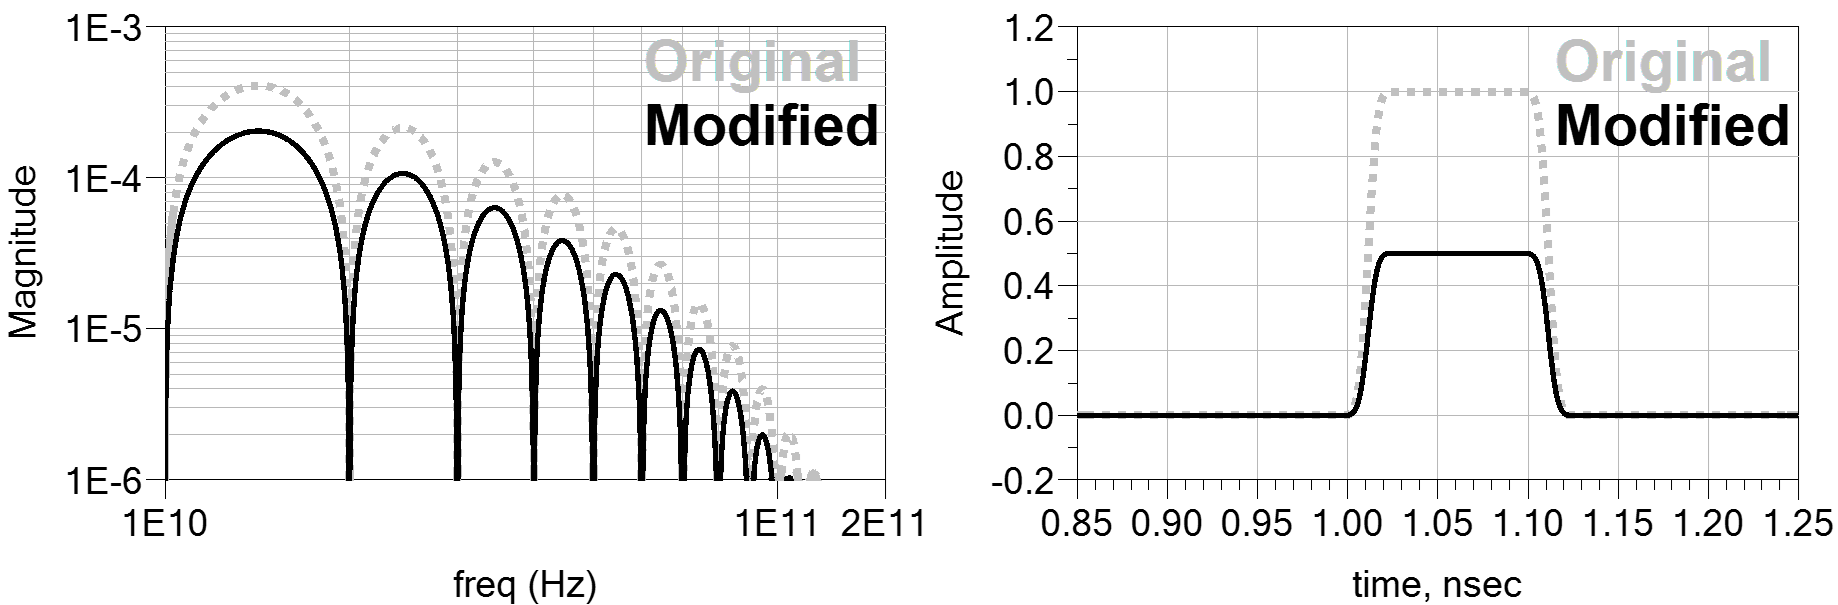
\includegraphics[width=0.9\textwidth]{Media/frekvensdoment_tidsdoment.png}
    \caption{Tids- og frekvensdomene av original og modifisert bølgeform. Pulsformen bestemmes av forholdet mellom frekvenskomponentene; er amplituder og relative faser like, blir tidskurven uendret.}
    \label{fig:eyediagram}
\end{figure}
\subsection{Dispersjon (fase, gruppeforsinkelse og gruppehastighet)}
Dispersjon beskrives av den imaginære delen av propagasjonskonstanten (fasekonstanten):
\[
    \beta_p(\omega)=\Im\{\gamma(\omega)\}
\]
Den sier noe om hvor mye hver frekvenskomponent forskyves i fase.
Fasen til kabelen er gitt ved:
\[
\varphi(\omega,l) = -\beta_p(\omega)\,l
\]
Fra fasen kan vi finne \emph{gruppeforsinkelse} og \emph{gruppehastighet}.
\emph{Gruppeforsinkelse} er definert som:
\[
\tau_g(\omega,l) = \varphi'(\omega,l) = -\frac{d}{d\omega}\varphi(\omega,l) = l\,\frac{d\beta_p(\omega)}{d\omega}
\]
Den sier noe om hvor mye en smal båndbredde rundt frekvensen \(\omega\) forsinkes i tid etter å ha passert kabelen. \emph{Gruppehastighet} er definert som:
\[
v_g(\omega) = \frac{1}{\tau_{g}'(\omega)} = \left(\frac{d\beta_p(\omega)}{d\omega}\right)^{-1}, \quad hvor \quad \tau_g'(\omega) = \frac{\tau_g(\omega,l)}{l} = \frac{d\beta_p(\omega)}{d\omega} \quad [\mathrm{s/m}]
\]
\clearpage
\noindent Den sier noe om hvor raskt en smal båndbredde rundt frekvensen \(\omega\) forplanter seg i kabelen. Det vi ser her er at \(\tau_g\) og \(v_g\) avhenger av frekvensen og det er netteopp dette som kalles \emph{dispersjon}. Vi kan tolke dette slik at ulike frekvenskomponenter av et signal forplanter seg med ulik hastighet. Dette får direkte konsekvenser for pulsform og øyediagram.\\
\begin{itemize}[leftmargin=2.8em,style=nextline]
  \item \textbf{Ingen dispersjon:} Hvis \(\frac{d\beta_p}{d\omega} \) er konstant (lineær fase), får alle frekvenskomponenter samme tidsforsinkelse \(\Rightarrow\) ingen pulsbredding (ingen horisontal øyelukking).\\
  \item \textbf{Dispersjon:} Når \(\frac{d\beta_p}{d\omega}\) varierer med frekvens (ikke-lineær fase), får ulike frekvenskomponenter ulik tidsforsinkelse \(\Rightarrow\) pulsbredding (horisontal øyelukking). I lavtap-tilfellet er ofte 
  \[
    \beta_p(\omega)\approx \omega\sqrt{LC}\quad,\quad slik\quad at \quad \tau_{g}'(\omega)=\frac{d\beta_p}{d\omega}\approx \sqrt{LC}\quad,\quad v_g(\omega)\approx \frac{1}{\sqrt{LC}}
  \]
  (nær konstant): da blir formen mest påvirket av demping, ikke fase-dispersjon.\\
\end{itemize}
\textbf{Spesialtilfelle (forvrengningsfri linje):}\\
Heaviside-betingelsen:
\[
    \alpha = \beta \quad \Rightarrow \quad \frac{R}{L}=\frac{G}{C}
\]
gir \(\beta_p(\omega)\) lineær i \(\omega\)
(konstant \(\tau_g'\)) og \(\alpha_p(\omega)\) frekvensuavhengig. Da fås ingen dispersiv forvrengning (kun lik demping av alle frekvenser).


\subsection{Kobling til pulstog}
Et periodisk innsignal med Fourierkoeffisienter \(c_n\) filtreres som
\[
f_{\text{out}}(t)=\Re\!\left\{\sum_{n=-N}^{N} c_n\,H(\omega_n,l)\,e^{j\omega_n t}\right\}.
\]
Demping (via \(\alpha_p\)) fjerner spesielt de høye leddene \(\Rightarrow\) langsommere kanter.\\
Dispersjon via: 
\[\frac{d\beta_p}{d\omega}\] 
tidsforskyver leddene relativt \(\Rightarrow\) pulsbredding.


\subsection{Oppsummering og kobling til prosjektet}

Teorien over forklarer hvorfor signaler i lange kabler dempes og forvrenges, og gir oss verktøyene til å analysere dette både analytisk og numerisk. Dette er avgjørende for å forstå hvorfor det er en anbefalt grense for Ethernet-kabler. I det videre arbeidet skal vi først gjennomføre praktiske målinger, og deretter \textcolor{red}{numeriske simuleringer} (kanskje), slik at begge kan sammenlignes med de teoretiske resultatene for å se hvordan modellen stemmer med virkeligheten.

\clearpage

\section{Metode}

\subsection{Mål og hypoteser}
\textbf{Formål:} analysere hvordan en transmisjonslinje (koaksialkabel) påvirker et pulstog i tids- og frekvensdomenet, og validere en RLCG-modell basert på telegrafligningen, numerisk simulering og laboratoriemålinger. Den estimerte overføringsfunksjonen predikerer målt demping og fase innenfor forhåndsdefinerte akseptgrenser. Overføringsfunksjonen:

\[
H(\omega) = e^{-\gamma(\omega)\ell} = e^{-\sqrt{(R+j\omega L)(G+j\omega C)}\,\ell}
\]

\subsection{Oversikt}
Metoden vi bruker i denne rapporten består av to hoveddeler: numerisk simulering og laboratoriestudie. Den numeriske simuleringen innebærer å modellere transmisjonslinjen ved hjelp av telegrafligningen. Vi bruker Python for å implementere denne modellen og generere simuleringsdata. I laboratoriestudien gjennomfører vi praktiske målinger av hvordan et pulstog påvirkes når det sendes gjennom en koaksialkabel av forskjellige lengder. Vi bruker en funksjonsgenerator til å generere pulstoget og et oscilloskop for å måle inngangs- og utgangssignaler.

\subsection{Numerisk simulering og modellering}
For å simulere telegrafligningen numerisk brukte vi Python med relevante biblioteker for numerisk beregning. Koden er vedlagt i vedlegg \ref{appendix:code}.

\paragraph{Modellantakelser.}
Vi modellerer kabelen som en lineær, tidsinvariant linje med fordelte parametre $R(f),L,C,G(f)$ per meter. Merk at $R$ og $G$ er frekvensavhengige for å modellere henholdsvis skinneffekt og dielektriske tap. Vi antar at kabelen er terminert med en last som matcher karakteristisk impedans, slik at vi kan se bort fra refleksjoner, i tillegg er verdier for $L$ og $C$ hentet fra datablad. Vi bruker funksjonen:
\[
\gamma(\omega)=\sqrt{(R+j\omega L)(G+j\omega C)},\qquad
H(\omega)=e^{-\gamma(\omega)\,\ell}
\]

\noindent Verdier for RGLC vil være følgende: \\
$R(f) = 0.17 \cdot \sqrt{\frac{f}{67 \cdot 10^3}} \qquad [\Omega / \mathrm{m}]$. \\
$L = 525 \mathrm{nH/m}$ \\
$C = 52 \mathrm{pF/m}$ \\
$G(f) = 2\pi f C \tan(\delta)$, \qquad $\tan(\delta) = 0.002$, \qquad [S/m]

\paragraph{Simuleringens modellering.}
Vi modellerer 5 forskjellige situasjoner for å forstå hvordan forskjellige medier påvirker signalet som propagerer gjennom. Lengdene på mediet er 10m, 50m, 100m og 1000m. Simuleringen tar utgangspunkt i formelen:
\[
\gamma (f) = \alpha(f) + j\beta(f), \qquad \gamma(f) = \gamma(\omega)|_{\omega = 2\pi f}
\]

\noindent Vi simulerer følgende modeller:
\begin{itemize}
    \item \textbf{Kun demping:} Ignorer faseendring ved å sette $\beta = 0$.
    \item \textbf{Kun faseendring:} Ignorer demping ved å sette $\alpha = 0$.
    \item \textbf{Ideell, tapsfri og ikke-dispersiv modell:} Mediet er ideelt, uten demping og uten dispersjon.
    \item \textbf{Full modell:} Inkluderer både demping og faseendring. Simuleringen tilnærmer seg virkeligheten.
    \item \textbf{Waterfall plott:} Simulerer hvordan forskjellige frekvenskomponenter påvirker tidsdomenesignalet.
\end{itemize}

\paragraph{Inngangssignal og representasjon.}
Vi modellerer pulstoget som en 50\% duty-cycle firkantpuls med periodetid $T = 2 \mu s$ og grunnvinkelhastighet $\omega_0 = 2\pi / T$. Siden duty-cycle er 50\% består spekteret av kun oddetalls harmoniske. Tidsfunksjonen representeres med Fourier-rekken.
\begin{equation}
    V_{\mathrm{in}}(t) = \frac{5}{2} + \sum_{\substack{n=-\infty\\ n\ \text{oddetall}}}^{N_{\mathrm{harm}}}\frac{5}{jn\pi} e^{jn\omega_0 t}
\end{equation} 

\subsection{Laboratoriestudie}
\paragraph{Gjennomførelse.} Dette er vårt praktiske forsøk for å studere og analysere telegrafligningen i virkeligheten. Vi bruker en funksjonsgenerator til å generere et firkant-pulstog som sendes gjennom en koaksialkabel av kjente forskjellige lengder. På mottakersiden bruker vi et oscilloskop for å sammenlikne data med en kort, direktekoblet koaksialkabel (referanse) og gjennom en lengre koaksialkabel.

\paragraph{Hensikt.} Hensikten med laberatorieforsøket er å undersøke hvordan signalet endres når det overføres gjennom en transmisjonslinje over forskjellige lengder. Ved høyere frekvenser forventes amplitudetap, faseforskyvning og forvrengning av signalet, som vi ønsker å kvantifisere og analysere.

\paragraph{Utstyr og oppsett.}
Utstyret i forsøket er følgende:
\begin{itemize}
    \item \textbf{Funksjonsgenerator.} Genererer firkant-pulstog med justerbar frekvens og amplitude. Firkant-pulstoget ble konfigurert til periodetid $T = 2 \mu s$ (frekvens $f_\mathrm{ref} = 500 \mathrm{kHz}$) med 50\% duty-cycle og amplitude på $2.5V_{pp}$. Startfasen ble satt til $0\si{\degree}$ for å sikre at signalet starter ved null.
    \item \textbf{Oscilloskop.} FFT-funksjonalitet for frekvensanalyse.
    \item \textbf{Kabler.} Koaksialkabel med lengder på 5m og 30m.
\end{itemize}

\paragraph{Måleprosedyrer.}
Måleprosedyrene inkluderer kalibrering av funksjonsgenerator og oscilloskop, oppsett av firkant-pulstog, og måling av inngangs- og utgangssignaler for hver kabellengde. På oscilloskopet målte vi $V_{in}$ og $V_{out}$ for hver kabellengde, og registrerte dataene for videre analyse. Her benyttet vi oss også av FFT (Fast Fourier Transform) for å analysere frekvensspekteret til signalene. Vi gjennomfører gjentatte målinger for å vurdere konsistens og usikkerhet.

\paragraph{FFT - Fast Fourier Transform.}
Vi benytter Fast Fourier Transform (FFT) på oscilloskopet for å konvertere tidsserier til frekvensdomenet og dermed studere systemets frekvensrespons. FFT er en effektiv algoritme for å beregne den diskrete Fourier-transformasjonen (DFT) og brukes blant annet i oscilloskopet for å vise frekvensspekteret. I motsetning til direkte DFT-beregning med kjøretid $O(N^2)$, har FFT kjøretid $O(N\log N)$, noe som muliggjør rask og effektiv analyse av store datasett og sanntidsmålinger.

\clearpage

\section{Modellering}
\subsection{Situasjon}
I den første modellen demonstrerer vi dempingen som de forskjellige< frekvenskomponentene i et signal opplever når det sendes gjennom et medium. Dette gjøres ved å sende et signal med flere frekvenskomponenter gjennom en dempende funksjon, og deretter analysere hvordan de forskjellige komponentene blir påvirket.
Vi tar utgangspunkt i en firkantpuls med periode $T$:
\[
    V_{in}(t) = \begin{cases}
        5, & -\frac{T}{2} \leq t < 0 \\
        0, & 0 \leq t < \frac{T}{2} \\
    \end{cases}, \quad hvor \quad T = 2 \mu s,\qquad duty\ cycle = 50\%
\]
Vi bestemmer først Fourier-rekken til firkantpulsen for å finne frekvenskomponentene:
\[
    V_{in}(t) = c_0 + \sum_{\substack{n=-\infty\\ n\ \text{oddetall}}}^{\infty} c_n e^{j n \omega_0 t}, \quad hvor \quad \omega_0 = \frac{2\pi}{T}
\]
Merk at siden vi vet at duty cycle er 50\%, vil bare oddetalls harmoniske være tilstede i Fourier-rekken.
Koefisientene $c_n$ kan beregnes som:
\[
    c_0 = \frac{1}{T} \int_{-T/2}^{T/2} V(t) dt = \frac{5}{2}
\]
\[
    c_n = \frac{1}{T} \int_{-T/2}^{T/2} V(t) e^{-j n \omega_0 t} dt =  \frac{5}{j 2 n \pi} (1 - (-1)^n)
\]
Vi for dermed at:
\[
    V_{in}(t) = \frac{5}{2} + \sum_{\substack{n=-\infty\\ n\ \text{oddetall}}}^{\infty} \frac{5}{j n \pi} e^{j n \omega_0 t}
\]
For å modellere dempingen i mediet, antar vi parametre som gir realistisk tilnærming til virkelige kabelverdier for R, G, L og C.
Vi antar at mediet er en Cat5e kabel med følgende parametere:
Fra formel \eqref{eq:skin-effekt} får vi at R er gitt ved:
\[
    R(f) = R_{DC} \cdot \sqrt{\frac{f}{f_{s}}}, \quad hvor \quad f_{s} = \frac{\rho_{cu}}{\pi \mu_{cu} r^2}, \quad R_{DC} = n_s \cdot \frac{\rho_{cu}}{\pi r^2}, \quad (merk\ at \quad \omega = 2\pi f)
\]
\[
    \rho_{cu} = 1.72 \cdot 10^{-8} \Omega m, \quad r = 0.255 mm, \quad \mu_{cu} = \mu_0 \cdot \mu_r = 4\pi \cdot 10^{-7} H/m., \quad n_s = 2
\]
\[
    f_s \approx 67kHz, \quad R_{DC} \approx 0.17 \Omega/m,
\]
Dermed får vi:
\[
    R(f) = 0.17 \cdot \sqrt{\frac{f}{67 \cdot 10^3}} \quad [\Omega/m]
\]
Vi antar videre at:
\[
    L = 525 nH/m, \quad C = 52 pF/m
\]
Fra formlen \eqref{eq:dielectric_loss} for dielektriske tap, får vi at:
\[
    G(f) = 2\pi f C \tan \delta, \quad hvor \quad \tan \delta = 0.002
\]
\clearpage
\noindent Vi står igjen med:
\[
    R(f) \approx 0.17 \cdot \sqrt{\frac{f}{67 \cdot 10^3}} \quad [\Omega/m], \quad L = 525 nH/m, \quad C = 52 pF/m, \quad G(f) \approx 0.65f \quad [pS/m]
\]

\noindent Vi har nå alt vi trenger for å finne overføringsfunksjonen til mediet:
\[
    H(f, l) = e^{-\gamma(f) l}, \quad hvor \quad \gamma(f) = \sqrt{(R(f) + j 2\pi f L)(G(f) + j 2\pi f C)}
\]
Her er $l$ lengden på mediet (kabelen) og $\gamma(f)$ er propagasjonskonstanten som avhenger av frekvensen.
Vi kan nå finne ut hvordan hver frekvenskomponent i firkantpulsen blir dempet ved å multiplisere hver komponent med $H(f, l)$:
\[
    V_{out}(t) = c_0H(0, l) + \sum_{\substack{n=-\infty\\ n\ \text{oddetall}}}^{\infty} c_n H(n f_0, l) e^{j n \omega_0 t}
\]
Som i denne situasjonen gir:
\[
    V_{out}(t) = \frac{5}{2}H(0, l) + \sum_{\substack{n=-\infty\\ n\ \text{oddetall}}}^{\infty} \frac{5}{j n \pi} H(n f_0, l) e^{j n \omega_0 t}    
\]
For å simulere dette numerisk, kan vi bruke Python til å beregne $H(f, l)$ for en rekke frekvenser og deretter rekonstruere tidsdomenesignalet ved hjelp av den inverse Fourier-transformasjonen.
Vi kan da plotte både inngangssignalet og utgangssignalet for å visualisere effekten av dempingen i mediet.
\clearpage
\subsection{Modeller}
For å forstå hvordan forskjellige aspekter av mediets egenskaper påvirker signalet, har vi laget flere modeller der vi varierer hvilke deler av den propagasjonskonstanten $\gamma(f)$ vi tar hensyn til. Modellene er basert på 10m, 50m, 100m og 1000m. Vi har følgende modeller:
\begin{itemize}
    \item \textbf{Kun demping:} I disse modellene tar vi kun hensyn til dempingen i mediet, og ignorerer faseendringen. Dette viser hvordan signalets amplitude påvirkes uten å endre dets form (modell 1 og 2).
    \[
        \gamma(f) = \alpha(f)
    \]
    \item \textbf{Kun faseendring:} I denne modellen tar vi kun hensyn til faseendringen i mediet, og ignorerer dempingen. Dette viser hvordan signalet ville oppføre seg i et ideelt tapsfritt medium (modell 3).
    \[
        \gamma(f) = j\beta(f)
    \]
    \item \textbf{Ideell, tapsfri og ikke-dispersiv modell:} Her antar vi at mediet er ideelt, uten demping og uten dispersjon. Dette betyr at alle frekvenskomponenter har samme fasehastighet (modell 4).
    \[
        \gamma(f) = j\beta(f), \quad hvor \quad \beta(f) = \omega\sqrt{LC}
    \]
    \item \textbf{Full modell:} Her tar vi hensyn til både demping (Re($\gamma$)) og faseendring (Im($\gamma$)) i mediet. Dette gir en tilnærmet representasjon av hvordan signalet påvirkes (modell 5).
    \[
        \gamma(f) = \alpha(f) + j\beta(f)
    \]
    \item \textbf{Waterfall plott:} For å visualisere hvordan forskjellige frekvenskomponenter påvirker tidsdomenesignalet, har vi laget to "waterfall" plot som viser hvordan signalet endres når vi inkluderer flere og flere frekvenskomponenter opp til en viss grensefrekvens (modell 6).
\end{itemize}
\clearpage
\subsection{Modell 1 (kun demping i frekvensdomenet)}
Demping av signalet er vist i figur \ref{fig:modell1}. Vi ser at høyfrekvente komponenter blir betydelig dempet, noe som resulterer i en mer avrundet firkantpuls ved utgangen. Dette illustrerer hvordan mediet fungerer som et lavpassfilter, hvor de høyere frekvensene reduseres mer enn de lavere frekvensene.
\begin{figure}[h]
    \centering
    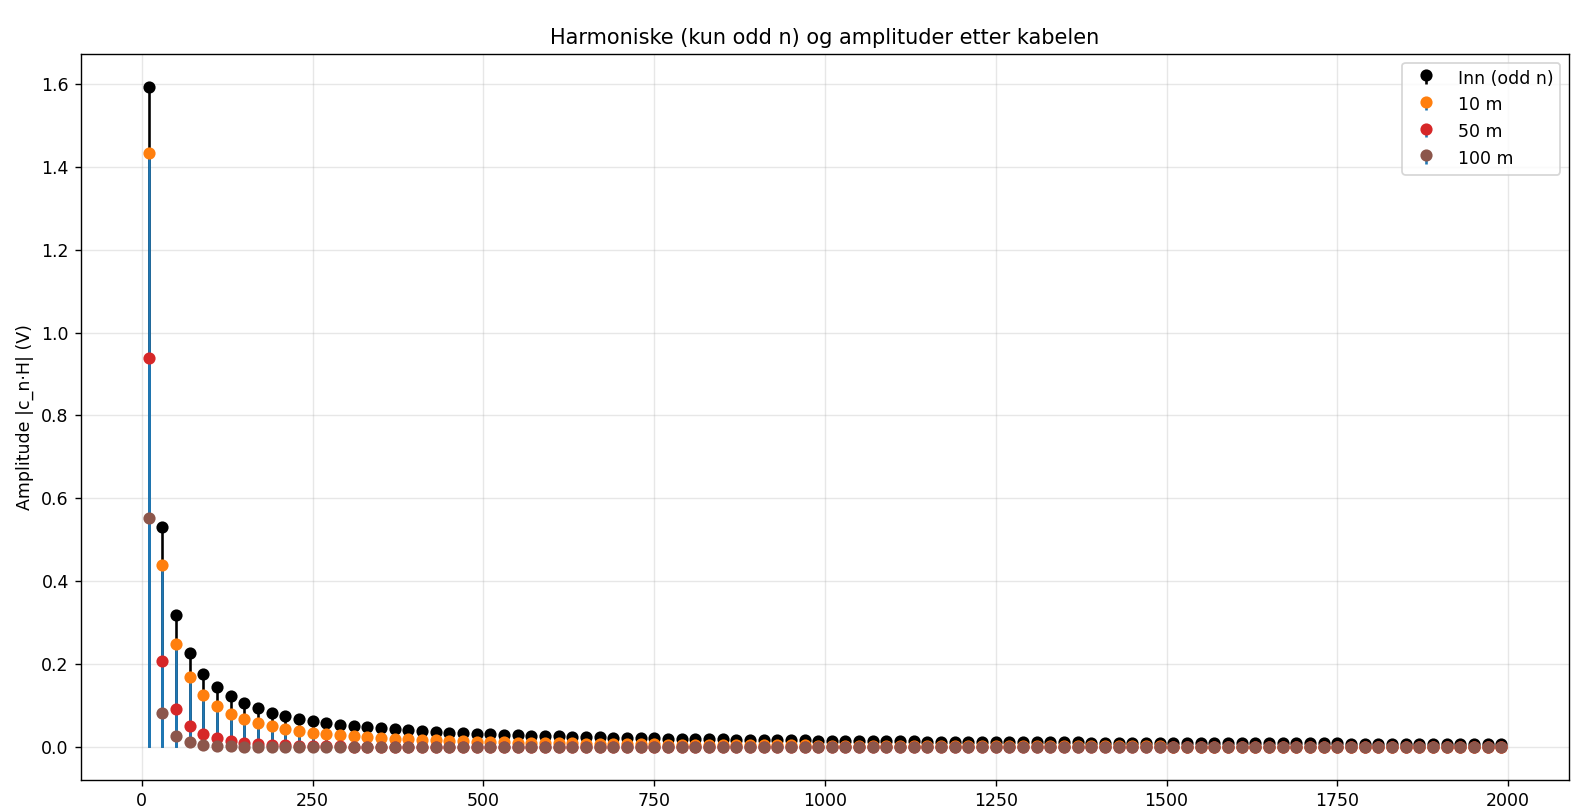
\includegraphics[width=1\textwidth]{Media/modellering1.png}
    \textit{
        \caption{Frekvensdomeneanalyse av firkantpuls etter å ha passert gjennom et dempende medium over forskjellige lengder.}}
    \label{fig:modell1}
\end{figure}
\clearpage
\subsection{Modell 2 (demping i frekvensdomenet i tidsdomenet)}
I den andre modellen ser vi på hvordan tidsdomenesignalet endres etter å ha passert gjennom mediet. Vi rekonstruerer tidsdomenesignalet ved å summere Fourier-rekkene for de dempede harmoniske. Her har vi kun tatt hensyn til amplitudendringen, og ikke faseendringen. Altså ser vi på:
\[
    H(f, l) = e^{-\alpha(f) l}, \quad hvor \quad \alpha(f) = Re(\gamma(f))
\]
Resultatet er vist i figur \ref{fig:modell2}. Vi ser at firkantpulsen blir mer avrundet etter å ha passert gjennom mediet, noe som bekrefter at høyfrekvente komponenter dempes mer enn lavfrekvente komponenter. Dette resulterer i en signifikant endring i signalets form, spesielt over lengre avstander.
\begin{figure}[h]
    \centering
    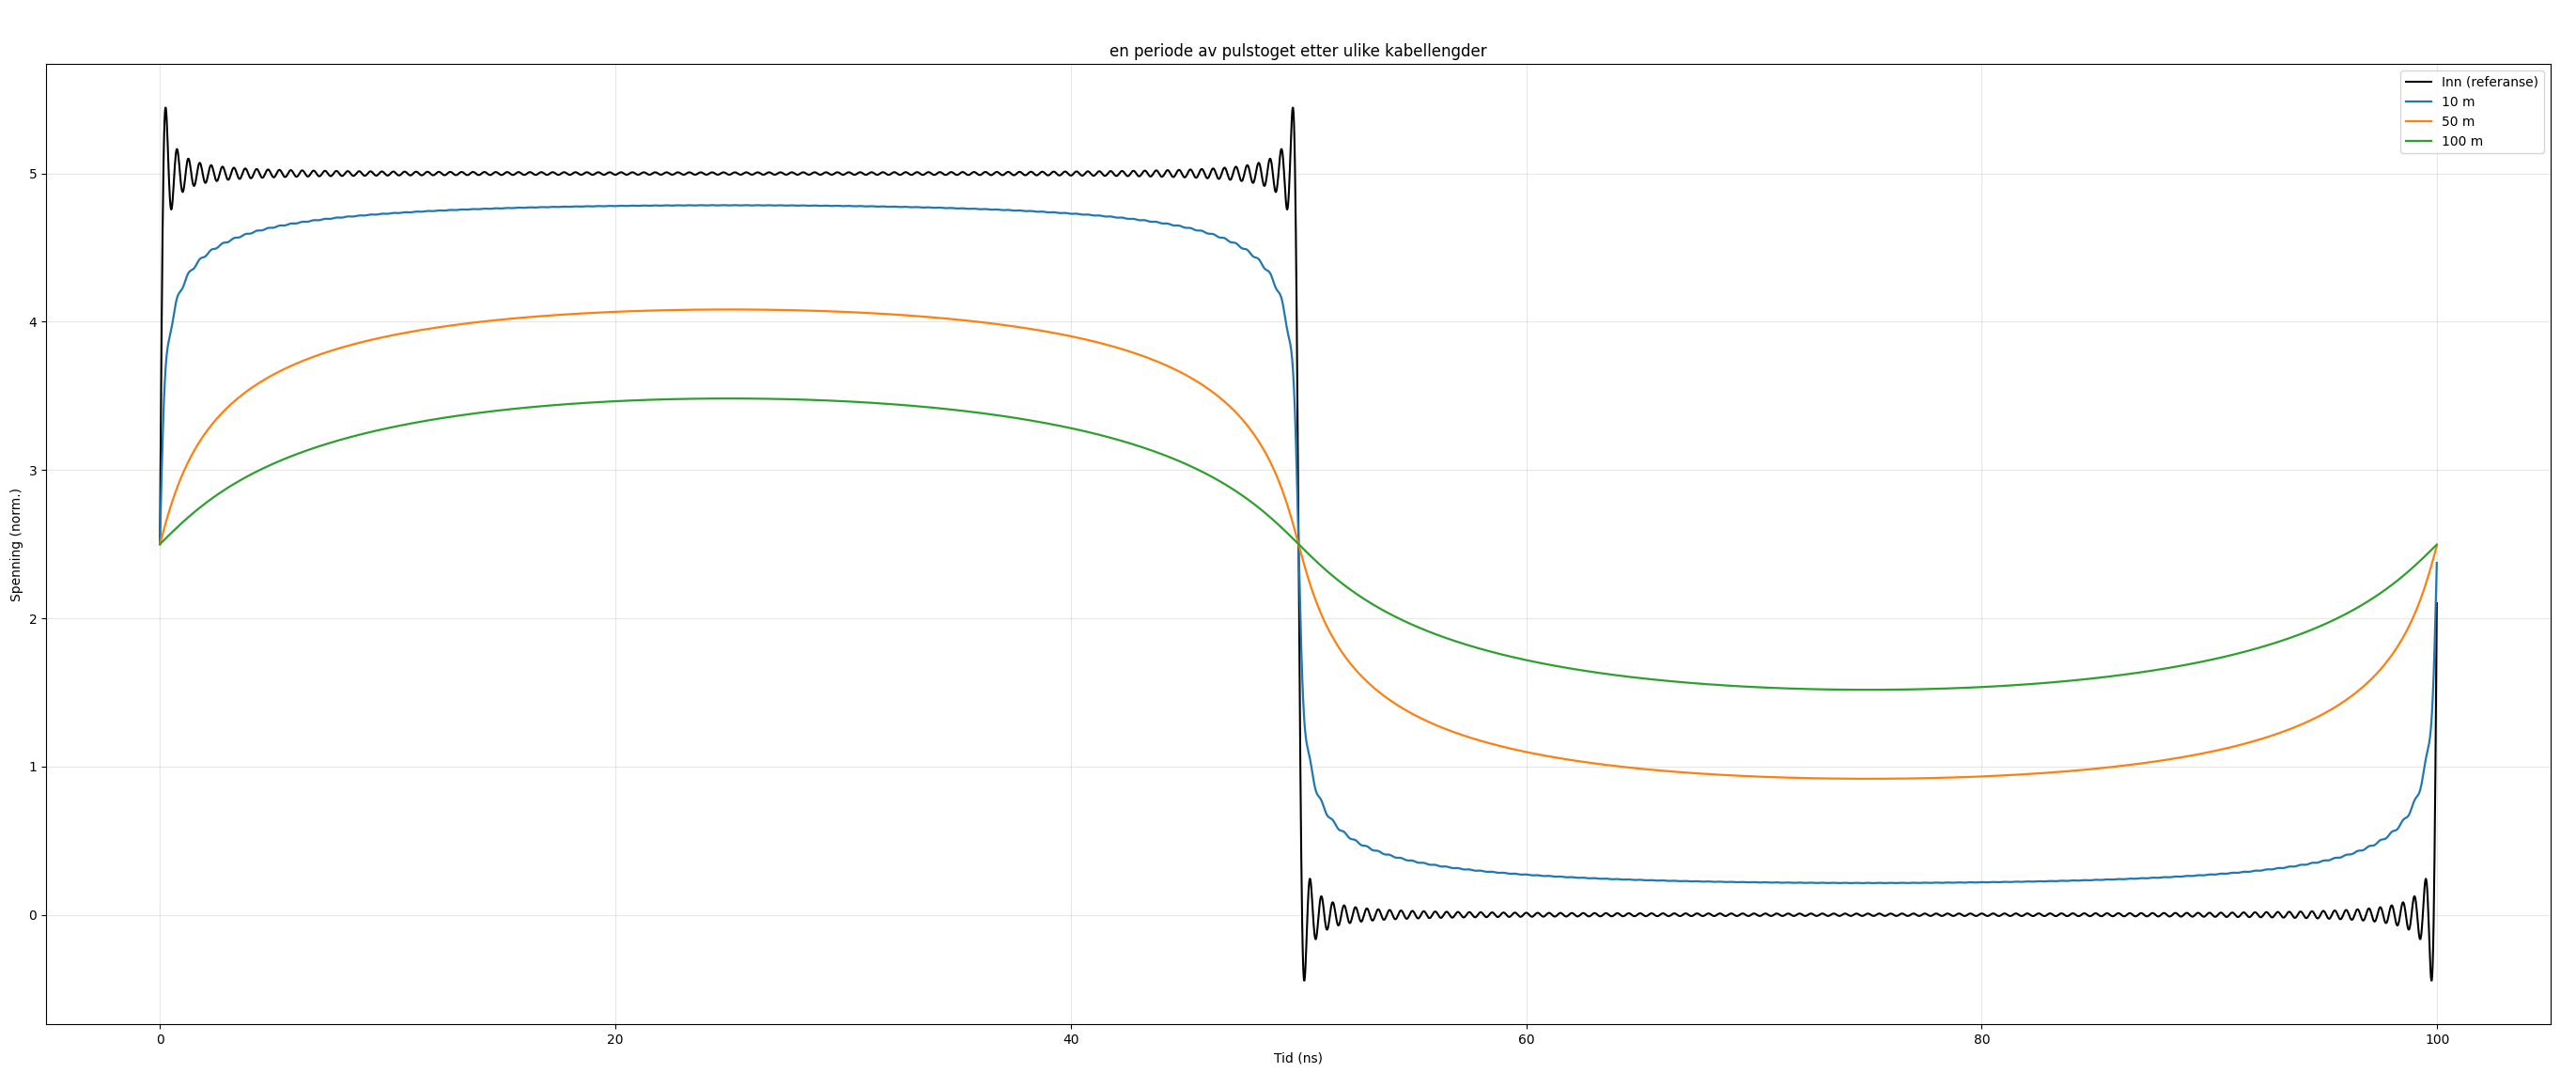
\includegraphics[width=1\textwidth]{Media/modellering2.png}
    \textit{
        \caption{Tidsdomenesignalet av firkantpuls etter å ha passert gjennom et dempende medium over forskjellige lengder.}}
    \label{fig:modell2}
\end{figure}
\clearpage
\subsection{Modell 3 (kun faseendring)}
I den tredje modellen ser vi på hvordan tidsdomenesignalet endres når vi kun tar hensyn til faseendringen i mediet, og ignorerer dempingen. Altså ser vi på:
\[
    H(f, l) = e^{-j\beta(f) l}, \quad hvor \quad \beta(f) = Im(\gamma(f))
\]
Resultatet er vist i figur \ref{fig:modell3}. Vi ser at firkantpulsen blir mer vrengete etter å ha passert gjennom mediet, men beholder sin generelle form. Dette illustrerer hvordan faseendringen påvirker signalets tidsdomenesignal uten å endre dets amplitude. Alle frekvenskomponenter opplever forskjellige faseforsinkelser, noe som fører til en forvrengning av signalets form.
\begin{figure}[h]
    \centering
    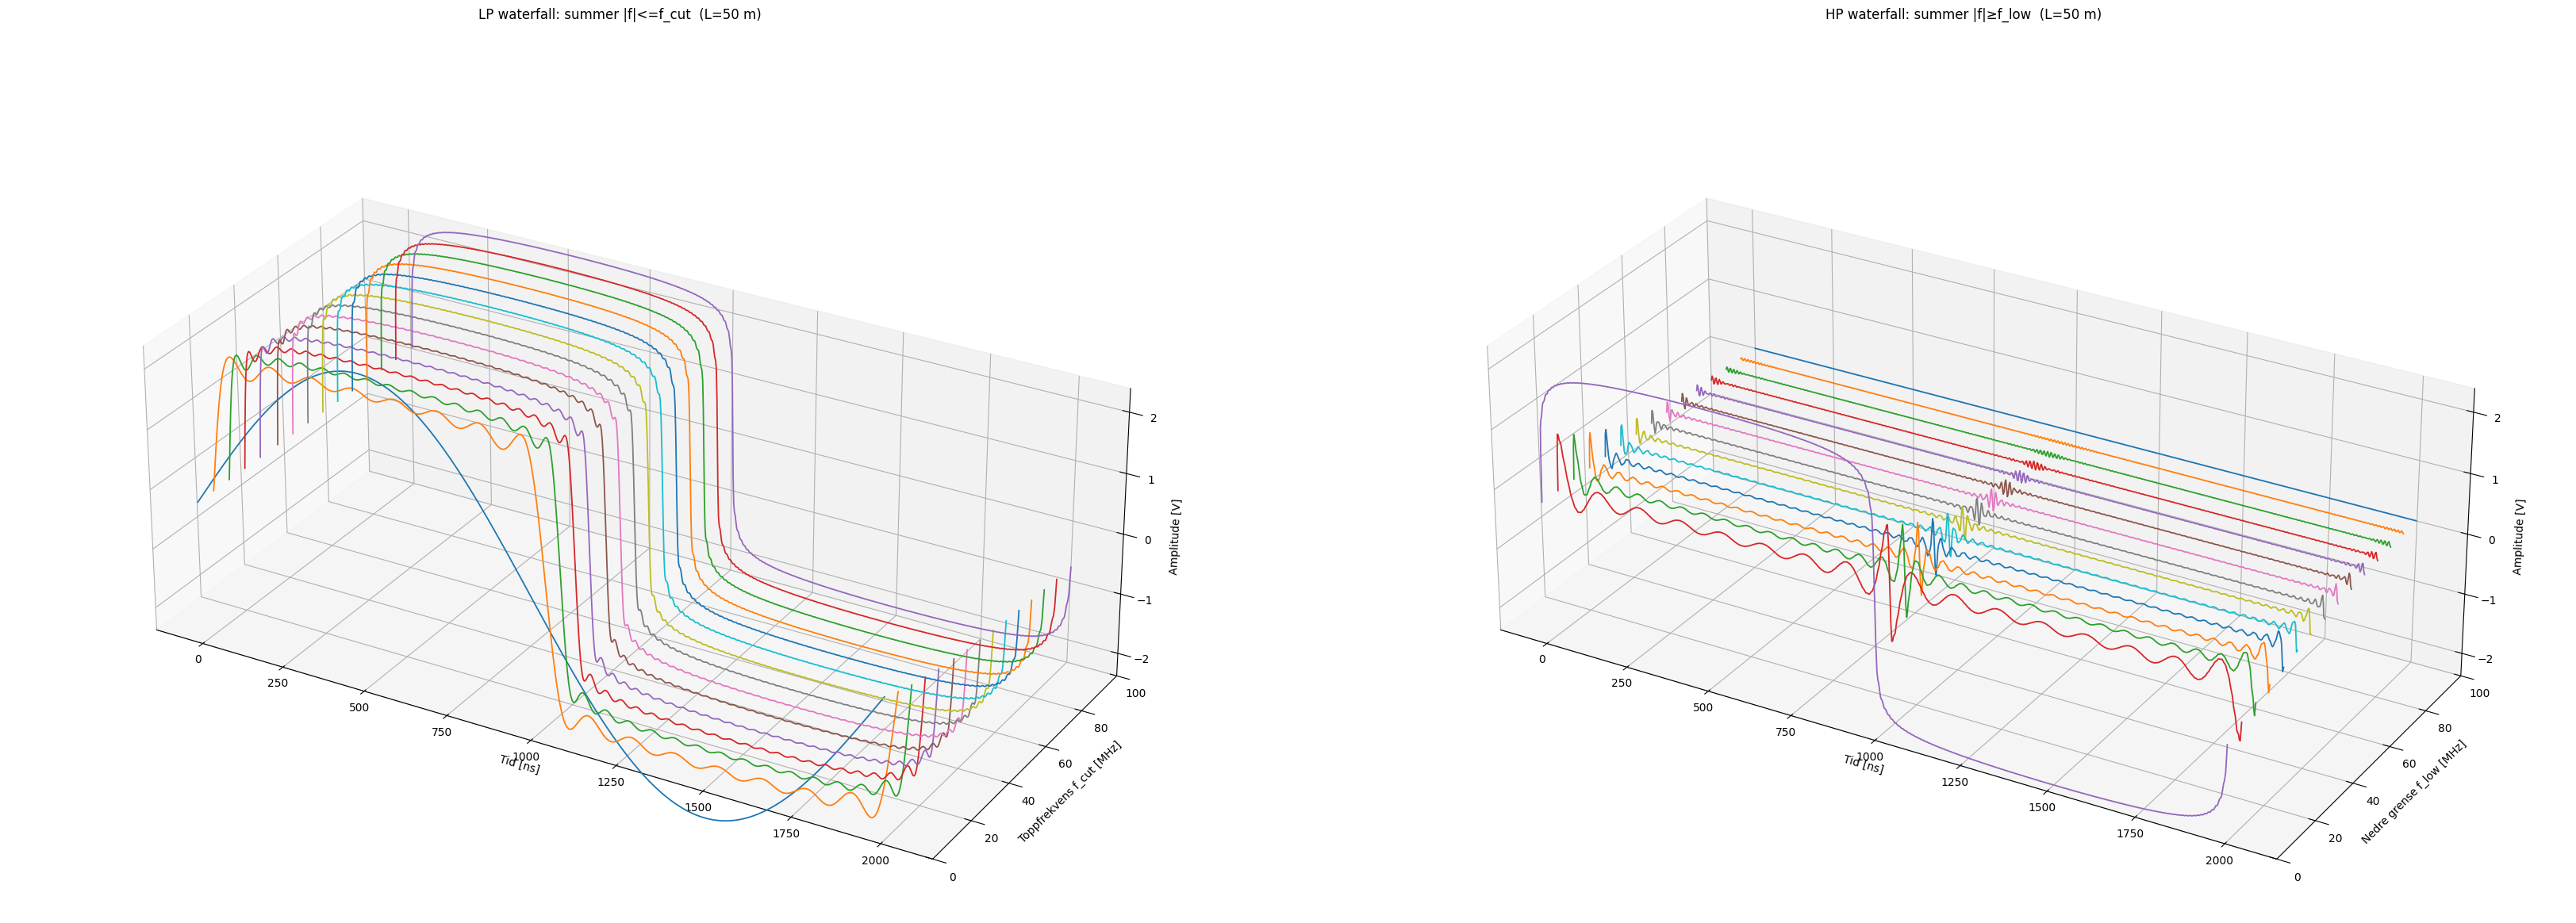
\includegraphics[width=1\textwidth]{Media/modellering3.png}
    \textit{
        \caption{Tidsdomenesignalet av firkantpuls etter å ha passert gjennom et medium med kun faseendring.}}
    \label{fig:modell3}
\end{figure}
\clearpage
\subsection{Modell 4 (Ideell, ikke-dispersiv modell)}
I den fjerde modellen ser vi på hvordan tidsdomenesignalet endres når vi antar at mediet er ideelt, uten demping og uten dispersjon. Altså ser vi på:
\[
    H(f, l) = e^{-j\beta(f) l}, \quad hvor \quad \beta(f) = \omega\sqrt{LC}
\]
Resultatet er vist i figur \ref{fig:modell4}. Vi ser at firkant
pulsen opprettholder sin opprinnelige form og blir forsinket i tid. Dette bekrefter at i et ideelt ikke-dispersivt medium, har alle frekvenskomponenter samme fasehastighet, noe som betyr at signalets form bevares uten noen forvrengning.
\begin{figure}[h]
    \centering
    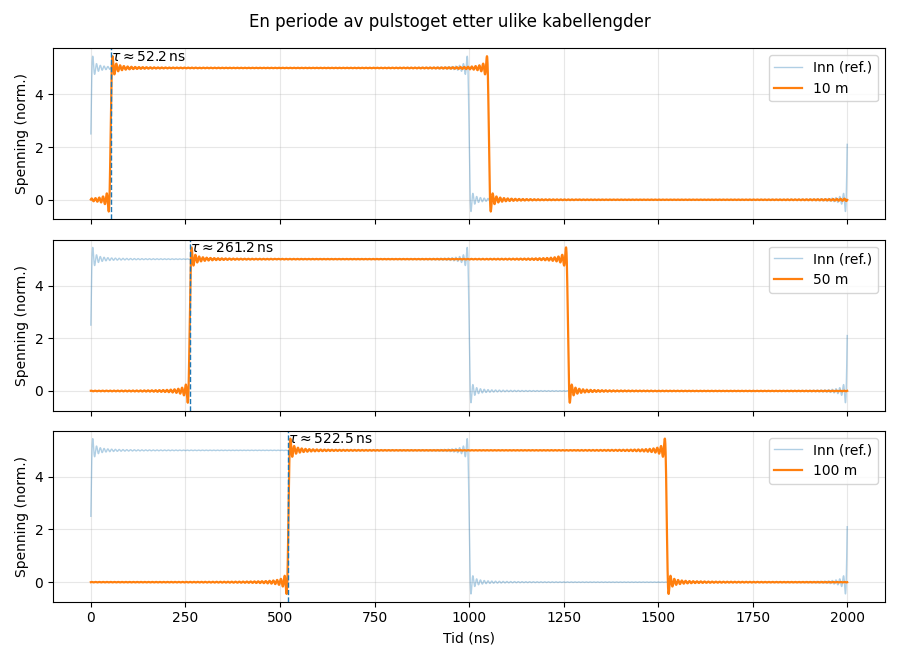
\includegraphics[width=1\textwidth]{Media/modellering4.png}
    \textit{
        \caption{Tidsdomenesignalet av firkantpuls etter å ha passert gjennom et ideelt ikke-dispersivt medium over forskjellige lengder.}}
    \label{fig:modell4}
\end{figure}
\clearpage
\subsection{Modell 5 (full modell)}
I den femte modellen ser vi på hvordan tidsdomenesignalet endres når vi tar hensyn til både demping og faseendring i mediet. Altså ser vi på:
\[
    H(f, l) = e^{-\gamma(f) l}, \quad hvor \quad \gamma(f) = \alpha(f) + j\beta(f)
\]
Resultatet er vist i figur \ref{fig:modell5}. Vi ser at firkantpulsen blir både dempet og forsinket i tid etter å ha passert gjennom mediet. Dette gir en mer realistisk representasjon av hvordan signalet påvirkes i et ekte medium, hvor både demping og faseendring spiller en rolle. Over lengre avstander blir signalet stadig mer forvrengt, noe som illustrerer viktigheten av å ta hensyn til begge aspekter for å forstå signalets oppførsel.
\begin{figure}[h]
    \centering
    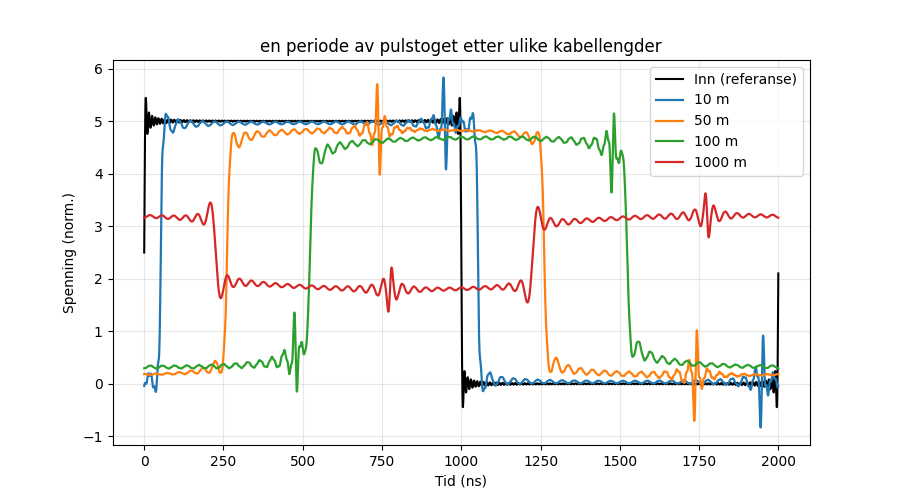
\includegraphics[width=1\textwidth]{Media/modellering5.png}
    \textit{
    \caption{Tidsdomenesignalet av firkantpuls etter å ha passert gjennom et realistisk medium over forskjellige lengder.}\label{fig:modell5}}
   
\end{figure}
\clearpage
\subsection{Modell 6 (Waterfall plot)}
For å få en bedre forståelse av hvordan forskjellige frekvenskomponenter påvirker tidsdomenesignalet, har vi laget to \textit{Waterfall} plot som viser hvordan signalet endres når vi inkluderer flere og flere frekvenskomponenter opp til en viss grensefrekvens (Visualisere bidraget fra hver komponent). Den ene kalles lavpassfilter (LP) og den andre høypassfilter (HP). Prinsippet er det samme for begge plottene, men de summerer forskjellige sett av frekvenskomponenter:
\begin{itemize}
    \item \textbf{Lavpassfilter (LP):} Her summerer vi alle frekvenskomponenter fra fundamentalfrekvensen $f_0$ opp til en økende grensefrekvens $f_{cut}$. Dette viser hvordan tidsdomenesignalet utvikler seg når vi inkluderer flere lavfrekvente komponenter.
    \[
        |f| \leq f_{cut}
    \]
    \item \textbf{Høypassfilter (HP):} Her summerer vi alle frekvenskomponenter fra en synkende grensefrekvens $f_{low}$ opp til en øvre grensefrekvens (for eksempel 100 MHz eller høyeste harmoniske). Dette viser hvordan tidsdomenesignalet påvirkes når vi inkluderer flere høyfrekvente komponenter.
    \[
        |f| \geq f_{low}
    \]
    \item \textbf{Antall kutt:} For å få en jevnere overgang i waterfall plottene, har vi økt antall kutt (cuts) til 13. Dette gir en mer detaljert visualisering av hvordan signalet endres med forskjellige grensefrekvenser.
\end{itemize}
Dette er vist i figur \ref{fig:modell6}.
\begin{figure}[h]
    \centering
    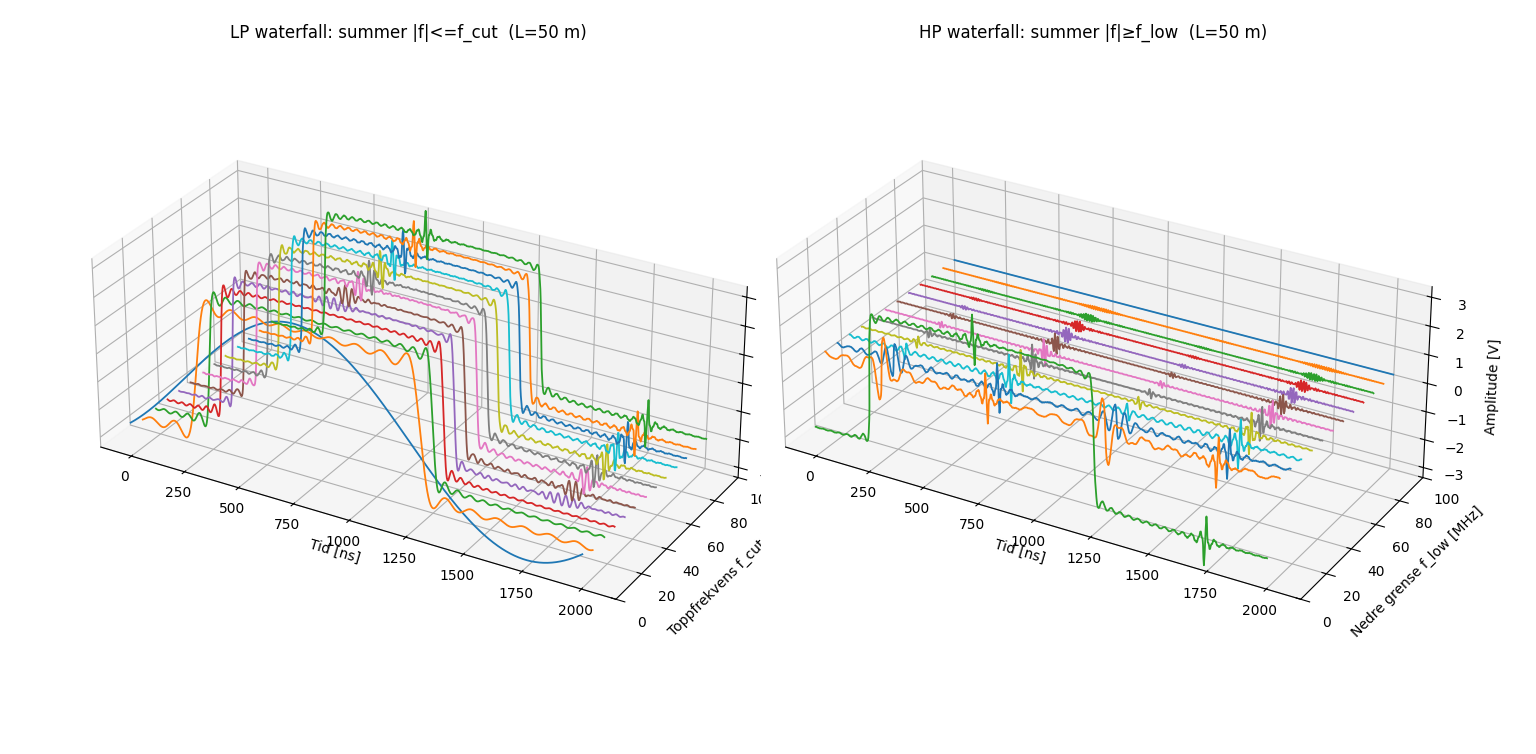
\includegraphics[width=1\textwidth]{Media/modellering6.png}
    \textit{
        \caption{Waterfall plot som viser hvordan tidsdomenesignalet endres når flere frekvenskomponenter inkluderes opp/ned til forskjellige grensefrekvenser (plottet er for 50m kabel).}\label{fig:modell6}}
    
\end{figure}\\
\clearpage
\noindent Vi ser at når vi inkluderer flere frekvenskomponenter, blir tidsdomenesignalet mer detaljert og nærmere den opprinnelige firkantpulsen. Dette illustrerer viktigheten av høyfrekvente komponenter for å bevare signalets form. For lavpassfilteret ser vi at signalet gradvis nærmer seg firkantpulsen når flere lavfrekvente komponenter inkluderes. For høypassfilteret ser vi at signalet blir mer avrundet når flere høyfrekvente komponenter inkluderes, noe som bekrefter at høyfrekvente komponenter er avgjørende for å opprettholde skarpe overganger i tidsdomenesignalet.
\clearpage


\clearpage

\section{Diskusjon}

\clearpage

\section{Konklusjon}
\dots

\clearpage

\nocite{*}
\printbibliography[heading=bibintoc,title={Referanser}]
\clearpage

\section*{Vedlegg}
\addcontentsline{toc}{section}{Vedlegg}
\section*{Vedlegg}\label{vedlegg}
\addcontentsline{toc}{section}{Vedlegg}
[1] GitHub repository for prosjektet: \\
\indent Url: \href{https://github.com/Yonatan1717/Project_Fourier-rekker}{\textcolor{blue}{https://github.com/Yonatan1717/Project\_Fourier-rekker}}\\
\indent Commit: \textcolor{blue}{87f30ac2ba8e7b7361574c4c5bfc16f0230a9cad} (commit fra 12.10.2025)\\
\indent Inneholder all kode og data brukt i prosjektet, mer informasjon i README.md filen.



\clearpage


\end{document}
